\documentclass[12pt]{article}
\usepackage{amsmath}
\usepackage{graphicx}
\usepackage{hyperref}
\usepackage[utf8]{inputenc}
\usepackage{geometry}
\usepackage{mathtools}
\usepackage{empheq}
\usepackage{listings}
\usepackage{xcolor}
\usepackage{authblk}
\usepackage{subcaption}

\graphicspath{ {./assets/} }
\geometry{margin=0.75in}

\title{CHEN 324 HW 2}
\author[1]{Zane Hernandez}
\author[2]{Bryce Gillilan}
\author[3]{Mark Levchenko}
\affil[1,2,3]{Group 11}
\date{January 2023}

\begin{document}
\maketitle
\newpage


\begin{enumerate}

% Problem 1 %%%%%%%%%%%%%%%%%%%%%%%%%%%%%%%%%%%%%%%%%%%%%%%%%%%%
    \item Problem 19.1-9
    \begin{enumerate}
        \item Derivation

        \begin{align*}
            N_B &= 0 \\
            N_A &= -c D_{AB} \frac{d x_A}{d z} + \frac{C_A}{c} (N_A + 0) \\
            N_A &= -c D_{AB} \frac{d x_A}{d z} + \frac{C_A}{c} N_A \\
            c &= \frac{P}{R T} \\
            P_A &= x_A P \\
            d x_A &= \frac{d P_A}{P} \\
            \frac{C_A}{c} &= \frac{P_A}{P} \\
            N_A &= -\frac{P}{R T} D_{AB} \frac{d P_A}{P d z} + \frac{P_A}{P} N_A \\
            N_A &= -\frac{D_{AB}}{R T} \frac{d P_A}{d z} + \frac{P_A}{P} N_A \\
            N_A \left(1 - \frac{P_A}{P} \right) &= -\frac{D_{AB}}{R T} \frac{d P_A}{d z} \\
            N_A \int_{z_1}^{z_2} dz  &= -\frac{D_{AB}}{R T} \int_{P_{A1}}^{P_{A2}} \frac{d P_A}{1 - \frac{P_A}{P}} \\
            N_A (z_2 - z_1) &= \frac{D_{AB} P}{R T} \ln{\left( \frac{P - P_{A2}}{P - P_{A1}} \right)} \\
            P_{BM} &= \frac{P_{A1} - P_{A2}}{\ln\left( \frac{P-P_{A2}}{P-P_{A1}} \right)} \\
            N_A (z_2 - z_1) &= \frac{D_{AB} P (P_{A1} - P_{A2})}{R T P_{BM}}  \\
            N_A &= \frac{\rho_A}{M_A} \frac{dz}{dt} \\
            r_1 &= z_2 - z_1 \\
            \frac{\rho_A}{M_A} \int_{r_2}^{r_1} r_1 dr &= \frac{D_{AB} P (P_{A1} - P_{A2})}{R T P_{BM}}  \int dt \\
            \frac{\rho_A}{2 M_A} (r_1^2 - r_2^2) &= \frac{D_{AB} P (P_{A1} - P_{A2})}{R T P_{BM}}  t_F \\
            r_2 & = 0 \\
            \frac{\rho_A}{2 M_A} r_1^2 &= \frac{D_{AB} P (P_{A1} - P_{A2})}{R T P_{BM}}  t_F
        \end{align*}
        \begin{equation*}
            \boxed{t_F = \frac{\rho_A R T P_{BM} r_1^2}{2 M_A D_{AB} P (P_{A1} - P_{A2})}}
        \end{equation*}
        \item Calculation
        \begin{align*}
            t_F &= \frac{\rho_A R T P_{BM} r^2}{2 M_A D_{AB} P (P_{A1} - P_{A2})} \\
            \rho_A &= 866 \\
            R &= 8.314 \\
            T &= 25.9 ^\circ \mathrm{C} = 299.05 \mathrm{K} \\
            P_{A1} &= 3.84 \\
            P_{A2} &= 0 \\
            P_{BM} &= \frac{3.82 - 0}{\ln\left( \frac{101.325 - 0}{101.325 - 3.84} \right)} = 99.39 \\
            r_1 &= 0.002 \\
            M_A &= 92.14 \\
            D_{AB} &= 0.086 \cdot 10^{-4} \\
            P &= 101.325 \\
            t_F &= \frac{866 \cdot 8.314 \cdot 299.05 \cdot 99.39 \cdot 0.002^2}{2 \cdot 92.14 \cdot 0.086 \cdot 10^{-4} \cdot 101.325 (3.84 - 0)} \\
            \Aboxed{t_F &= 1388.2 \mathrm{s}}
        \end{align*}
    \end{enumerate}

% Problem 2 %%%%%%%%%%%%%%%%%%%%%%%%%%%%%%%%%%%%%%%%%%%%%
\newpage
    \item Problem 19.1-21
    \begin{enumerate}
        \item 

        \begin{equation*}
            \mathrm{2A} \rightarrow \mathrm{B}
        \end{equation*}
        \begin{align*}
            \frac{d C_A}{t} &= -\nabla N_A + r_A \\
            \intertext{Steady state}
            -\nabla N_A + r_A &= 0 \\
            N_A &= -D_{AB}\frac{d C_A}{dz} + x_A N_T \\
            \frac{1}{2} N_A &= -N_B \\
            N_T &= N_A - \frac{1}{2} N_A \\
            N_T &= \frac{1}{2} N_A \\
            N_A &= -D_{AB}\frac{d C_A}{dz} + \frac{1}{2} N_A x_A \\
            N_A &= \frac{-D_{AB} C dx_A}{(1-\frac{x_A}{2}) dz} \\
            N_A \int dz &= -D_{AB} C \int \frac{dx_A}{1-\frac{x_A}{2}} \\
            C &= \frac{P}{RT} \\
            \Aboxed{N_A &= \frac{2 D_{AB} P}{\delta R T} \ln\left( \frac{x_{A2} - 2}{x_{A1} - 2} \right)}
        \end{align*}
        
        \item Calculation
        \begin{align*}
            D_{AB} &= 0.2 \cdot 10^{-4} \\
            P &= 101.32 \\
            X_{A1} &= 0.97 \\
            X_{A2} &= 0 \\
            \delta &= 0.0013 \\
            R &= 8.314 \\
            T &= 298 \\
            N_A &= \frac{2 \cdot 0.2 \cdot 10^{-4} \cdot 101.32}{0.0013 \cdot 8.314 \cdot 298} \ln\left( \frac{0 - 2}{0.97 - 2} \right) \\
            \Aboxed{N_A &= 8.35 \cdot 10^{-4}\mathrm{\frac{kgmol}{m^2 \cdot s}}}
        \end{align*}

        \item Finite reaction rate
        \begin{align*}
            N_A A_s &= k_1' C_{A2} V_L \\
            C_{A2} &= \frac{x_{A2} P}{RT} \\
            N_A A_s &= k_1' \frac{x_{A2} P}{RT} V_L \\
            x_{A2} &= \frac{N_A A_s RT}{k_1' P V_L} \\
            N_A &= \frac{2 D_{AB} P}{\delta R T} \ln\left( \frac{x_{A2} - 2}{x_{A1} - 2} \right) \\
            \Aboxed{N_A &= \frac{2 D_{AB} P}{\delta R T} \ln\left( \frac{\frac{N_A A_s RT}{k_1' P V_L} - 2}{x_{A1} - 2} \right)}
        \end{align*}

        \item Calculation
        \begin{align*}
            N_A &= \frac{2 D_{AB} P}{\delta R T} \ln\left( \frac{\frac{N_A A_s RT}{k_1' P V_L} - 2}{x_{A1} - 2} \right) \\
            D_{AB} &= 0.2 \cdot 10^{-4} \\
            P &= 101.32 \\
            X_{A1} &= 0.97 \\
            X_{A2} &= 0 \\
            \delta &= 0.0013 \\
            R &= 8.314 \\
            T &= 298 \\
            k_1' &= 0.53 \cdot 10^{-2} \\
            \intertext{Solve the system}
            \Aboxed{N_A &= 1.766 \cdot 10^{-4}\mathrm{\frac{kgmol}{m^2 \cdot s}}}
        \end{align*}
    \end{enumerate}


% Problem 3 %%%%%%%%%%%%%%%%%%%%%%%%%%%%%%%%%%%%%%%%%%%%%
\newpage
    \item Problem 19.3-1
    \begin{align*}
        \intertext{Steady state no reaction}
        N_A &= \frac{D_{AB} C}{1 - x_A} \frac{dx_A}{dz} \\
        N_A &= \frac{D_{AB} C}{\delta x_{BM}} (x_{A1} - x_{A2}) \\
        N_A &= \frac{D_{AB}}{\delta x_{BM}} (C_{A1} - C_{A2}) \\
        C_A &= \frac{S P_A}{22.414} \\
        x_{BM} &= 1 \\
        N_A &= \frac{D_{AB} S}{t_M 22.414} (P_{A1} - P_{A2}) \\
        D_{AB} &= 0.11 \cdot 10^{-9} \\
        S &= 0.90 \\
        t_M &= 0.030 \\
        P_{A1} &= 2 \\
        P_{A2} &= 1 \\
        A_c &= 4 \cdot 10^{-4} \\
        N_A &= \frac{D_{AB} S}{t_M 22.414} (P_{A1} - P_{A2}) \\
        N_A &= \frac{D_{AB} S}{t_M 22.414} (P_{A1} - P_{A2}) A_c \\
        N_A &= \frac{0.11 \cdot 10^{-9} \cdot 0.90}{0.030 \cdot 22.414} (2 - 0) \cdot 4 \cdot 10^{-4} \\
        \Aboxed{N_A &= 1.1778 \cdot 10^{-13}\mathrm{\frac{kgmol(CO_2)}{m^2 \cdot s}}}
    \end{align*}

% Problem 4 %%%%%%%%%%%%%%%%%%%%%%%%%%%%%%%%%%%%%%%%%%%%%
\newpage
    \item Problem 20.10-4
    \begin{align*}
        \intertext{Convection resistance is zero}
        \frac{k_c}{D_{AB}} \sqrt{D_{AB} t} &= \infty \\
        t &= 3600 \\
        C_0 &= 0.14 \\
        C_1 &= 0.03 \\
        \intertext{for $x=0.005$m}
        \frac{x}{2\sqrt{D_{AB} t}} &= \frac{0.005}{2\sqrt{1.29 \cdot 10^{-8} \cdot 3600}} = 0.367 \\
        \intertext{From Figure 14.3-3}
        \frac{C - C_0}{C_1 - C_0} &\approx 0.6 \\
        \frac{C - 0.14}{0.03 - 0.14} &= 0.6 \\
        \Aboxed{C &= 0.074} \\
        \intertext{for $x=0.01$m}
        \frac{x}{2\sqrt{D_{AB} t}} &= \frac{0.01}{2\sqrt{1.29 \cdot 10^{-8} \cdot 3600}} = 0.734 \\
        \intertext{From Figure 14.3-3}
        \frac{C - C_0}{C_1 - C_0} &\approx 0.28 \\
        \frac{C - 0.14}{0.03 - 0.14} &= 0.28 \\
        \Aboxed{C &= 0.109} \\
        \intertext{for $x=0.02$m}
        \frac{x}{2\sqrt{D_{AB} t}} &= \frac{0.02}{2\sqrt{1.29 \cdot 10^{-8} \cdot 3600}} = 1.467 \\
        \intertext{From Figure 14.3-3}
        \frac{C - C_0}{C_1 - C_0} &\approx 0.039 \\
        \frac{C - 0.14}{0.03 - 0.14} &= 0.039 \\
        \Aboxed{C &= 0.136} \\
    \end{align*}

    Plot of depth v weight\%:
    
    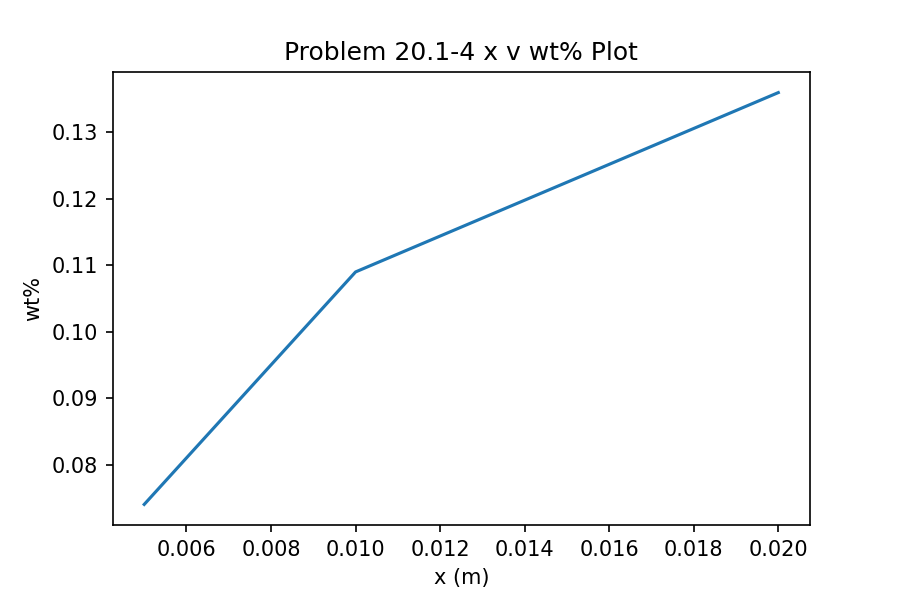
\includegraphics[]{Problem 20.1-4 fig.png}
\end{enumerate}
\end{document}
